\frame{
	\frametitle{Indexing Definitions}

	\begin{description}
		\item[$I(A, b)_k$:] index of k\textsuperscript{th} occurrence of b in A
		\item[$\beta_i$:] $\#$ of v's between i\textsuperscript{th} and (i+1)\textsuperscript{th} h collisions: $[I(\alpha, h)]_{i+1} - [I(\alpha, h)]_{i} - 1$
	\end{description}

	\begin{example}
		\begin{align*}
			\alpha& = hvvvvhvvvvhvvvh\\
			I(\alpha, h)& = (0, 5, 10, 14)\\
			\beta& = (4, 4, 3)
		\end{align*}
	\end{example}
}

\frame{
	\frametitle{First Indexing Theorem}

	\begin{theorem}
		\[
			\beta_i \ge 1 \qquad \forall \; i \in \cbracket{0, \dotsc, length(I(\alpha, h))-2}
		\]
	\end{theorem}

	\pause

	\begin{example}
		\begin{itemize}
			\item $\alpha = hvvhhvvvhvvhhvhhvvvvhvvvh \qquad \beta = (2, 0, 3, 2, 0, 1, 2, 4, 3)$
			\item $\alpha = hvvvvhvvvvhvhvvvhvvvvvvvh \qquad \beta = (4, 4, 1, 3, 7)$
			\item $\alpha = hvvvvhvvvvhvvvhvvvvhvvvvh \qquad \beta = (4, 4, 3, 4, 4)$
		\end{itemize}
	\end{example}
}

\frame{
	\frametitle{First Indexing Theorem}

	\begin{theorem}
		\[
			\beta_i \ge 1 \qquad \forall \; i \in \cbracket{0, \dotsc, length(I(\alpha, h))-2}
		\]
	\end{theorem}

	\begin{example}
		\begin{itemize}
			\item \sout{$\alpha = hvvhhvvvhvvhhvhhvvvvhvvvh \qquad \beta = (2, 0, 3, 2, 0, 1, 2, 4, 3)$}
			\item $\alpha = hvvvvhvvvvhvhvvvhvvvvvvvh \qquad \beta = (4, 4, 1, 3, 7)$
			\item $\alpha = hvvvvhvvvvhvvvhvvvvhvvvvh \qquad \beta = (4, 4, 3, 4, 4)$
		\end{itemize}
	\end{example}
}

\frame{
	\frametitle{Parametric Representation}

	\begin{figure}
    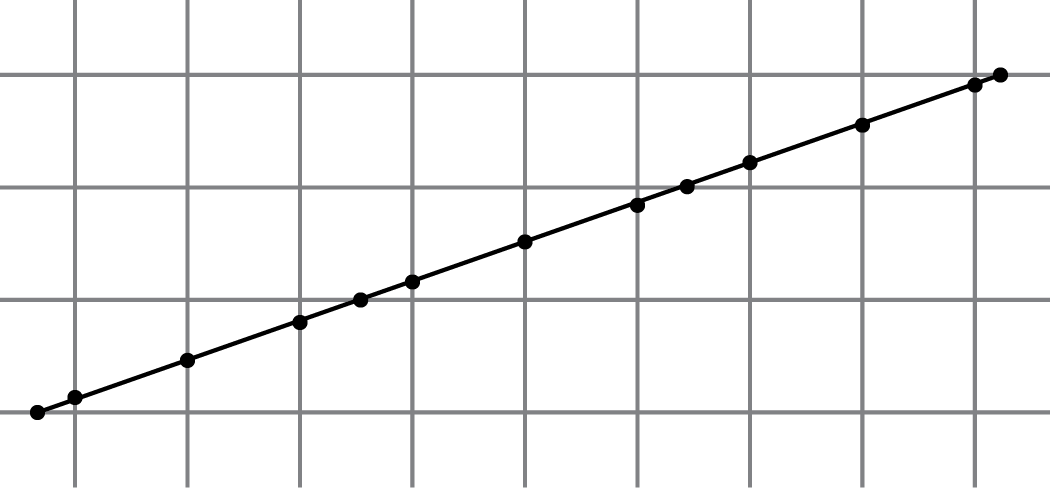
\includegraphics[width=3in]{1d-mapping_1}
  \end{figure}
}

\frame{
	\frametitle{Parametric Representation}

	\begin{figure}
    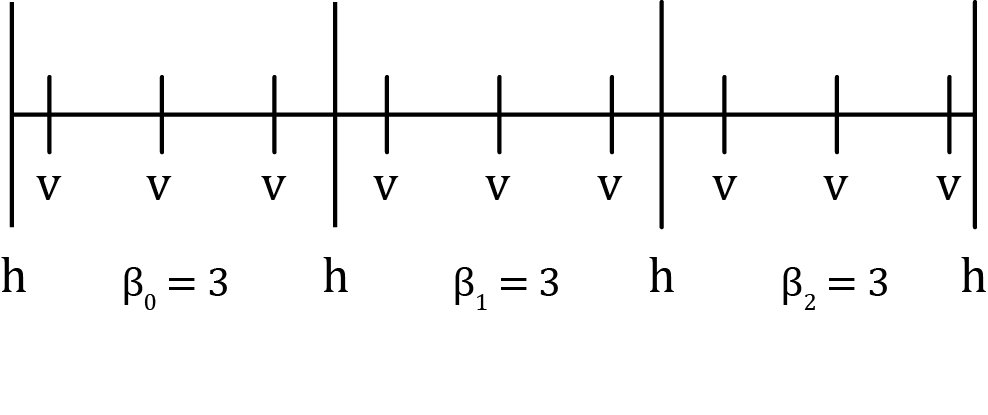
\includegraphics[width=3in]{1d-mapping_2}
  \end{figure}
}

\frame{
	\frametitle{Parametric Representation}

	\begin{figure}
    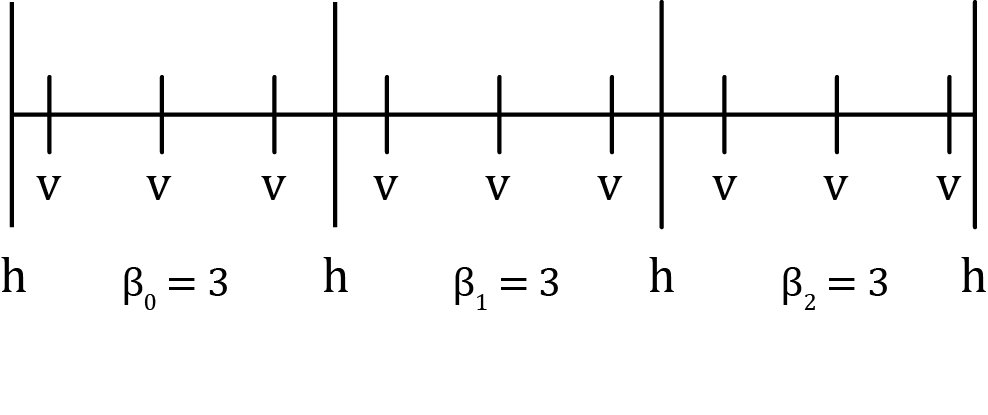
\includegraphics[width=3in]{1d-mapping_3}
  \end{figure}
}